\documentclass[a4paper,10pt]{article}

% IMPORTS
\usepackage{amsfonts}
\usepackage{amsmath}
\usepackage{amssymb}
\usepackage{graphicx}
\usepackage{titlesec}
\usepackage{wrapfig}
\usepackage[ngerman]{babel}
\usepackage[utf8x]{inputenc}
\usepackage{pdfpages}
\usepackage{placeins}
\usepackage{color}
\usepackage{eurosym}
\usepackage{xargs}
\usepackage{xcolor}
\usepackage{subcaption}
\usepackage{hyperref}
\usepackage[margin=2cm]{geometry}
\usepackage{enumitem}
\usepackage{float}
\usepackage[colorinlistoftodos,prependcaption,textsize=tiny]{todonotes}

% CONFIG
\clubpenalty = 9000
\widowpenalty = 9000
\displaywidowpenalty = 9000
\titlespacing\subsection{0pt}{14pt plus 4pt minus 2pt}{2pt plus 2pt minus 1pt}
\titlespacing\subsection{0pt}{10pt plus 4pt minus 2pt}{2pt plus 2pt minus 1pt}
\setlength{\parindent}{0pt}
\setcounter{tocdepth}{2}

% -----------------------------------------------------------------------------
\begin{document}

\begin{center}
	\huge Mitschrift der 1. Klausur zum \\
	\Huge \textbf{Basiskurs Mathematik} \\
	\huge bei Prof. Kreuzer im WS 16/17 \\
	\normalsize

	\vspace{.5cm}
	\begin{tabular}[b]{l|l}
		\textbf{Author} & NF \\ %Niko Fink \texttt{<finksim@fim.uni-passau.de>} \\
		\textbf{Datum} & 14.02.2017 \\
		\textbf{Hilfsmittel} & keine \\
		\textbf{Dauer} & $120+ min$ \\
		\textbf{Punkte} & alle Aufgaben brachten gleich viele Punkte \\
		\textbf{letzte Änderung} & \today \\
	\end{tabular}

	\vspace{.5cm}
\end{center}

\renewcommand\thesection{}
\renewcommand\thesubsection{\arabic{subsection}.}

\section{Klausur}

\subsection{Aufgabe}
Bestimmen Sie alle ganzzahligen Lösung der Gleichung $x^2+9xy+y^2=6$.

\subsection{Aufgabe}
\begin{enumerate}[label=\alph*)]
\item Stellen Sie $x^4+x^2+1$ als Produkt zweier quadratischer Polynome dar.
\item Bestimmen Sie alle $z \in \mathbb{C}$ mit $z^4+z^2+1=0$ und stellen Sie sie in der Form $z = x + y i$ dar.
\end{enumerate}

\subsection{Aufgabe}
Bestimmen Sie alle reellen Lösungen der Ungleichung $|2x + 1| - |2x| + 1 = 2x$.

\subsection{Aufgabe}
Gegeben sei ein Dreieck $ABC$ und Punkte $D,M,P$. Hierbei gelte:
\begin{enumerate}
\item $M$ ist der Umkreismittelpunkt von $ABC$ und liegt auf $\overline{AB}$.
\item $AB$ steht senkrecht zu $CM$.
\item $D$ liegt auf dem Umkreis von $ABC$, und zwar so auf dem kürzeren Bogen von $A$ nach $C$, dass $\measuredangle MDB=15^\circ$.
\item $P$ liegt auf $\overline{MC}$ und $AB$ ist parallel zu $DP$.
\end{enumerate}
Aufgaben:
\begin{enumerate}[label=\alph*)]
\item Erstellen Sie eine Planfigur mit den oben genannten Eigenschaften.
\item Zeigen Sie, dass das Dreieck $MCD$ gleichseitig ist.
\item Berechnen Sie $\overline{PC}$ in Abhängigkeit von $\overline{AB}$.
\end{enumerate}

\subsection{Aufgabe}
Sei $ABC$ ein gleichschenkliges Dreieck mit der Basis $\overline{AB} = 2cm$.\\
$D$ sei die dritte Ecke des gleichschenkligen (rechtwinkeligen) Dreiecks $ACD$ mit $\measuredangle DCA=90^\circ$.\\
$E$ sei die dritte Ecke des gleichschenkligen (rechtwinkeligen) Dreiecks $BEC$ mit $\measuredangle BCE=90^\circ$.
\begin{enumerate}[label=\alph*)]
\item Fertigen Sie eine Skizze an.
\item Zeigen Sie, dass $DE$ parallel zu $AB$ ist.
\item Berechnen Sie den Flächeninhalt des Vierecks $ABED$ in Abhängigkeit von der Höhe von $\triangle ABC$ und der Basis $\overline{AB}$.
\end{enumerate}

\subsection{Aufgabe}
Bestimmen Sie $\tan(22,5^\circ)$.

\section{Lösungsskizze}

\subsection{Aufgabe} %1
\begin{figure}[h!]
	\centering
	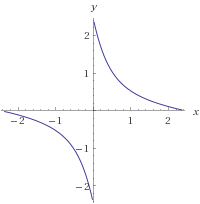
\includegraphics[width=.3\linewidth]{res/KL161-1.png}
\end{figure}

\subsection{Aufgabe} %2
\begin{align*}
x^4+x^2+1 &= (x^2+1)x^2 + 1 = (x^2 + 1)^2 - x^2\text{ \textit{hilft nicht}} \\
(x^2-x+1)(x^2+x+1) &= (x^2-(x-1))(x^2+(x+1)) \\
&= \left(x^2\right)^2 + (x+1)x^2 - (x-1)x^2 - (x+1)(x-1) \\
&= x^4 + x^2 (x+1-(x-1)) - x^2 + 1^2 \\
&= x^4 + 2x^2 - x^2 + 1 \\
&= x^4 + x^2 + 1
\end{align*}

\subsection{Aufgabe} %3
\[|2x + 1| - |2x| + 1 = 2x \Leftrightarrow x=1\]
\begin{figure}[H]
	\centering
	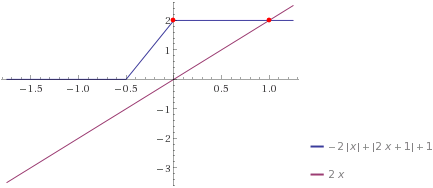
\includegraphics[width=.5\linewidth]{res/KL161-3.png}
\end{figure}

\subsection{Aufgabe} %4
\begin{figure}[H]
	\centering
	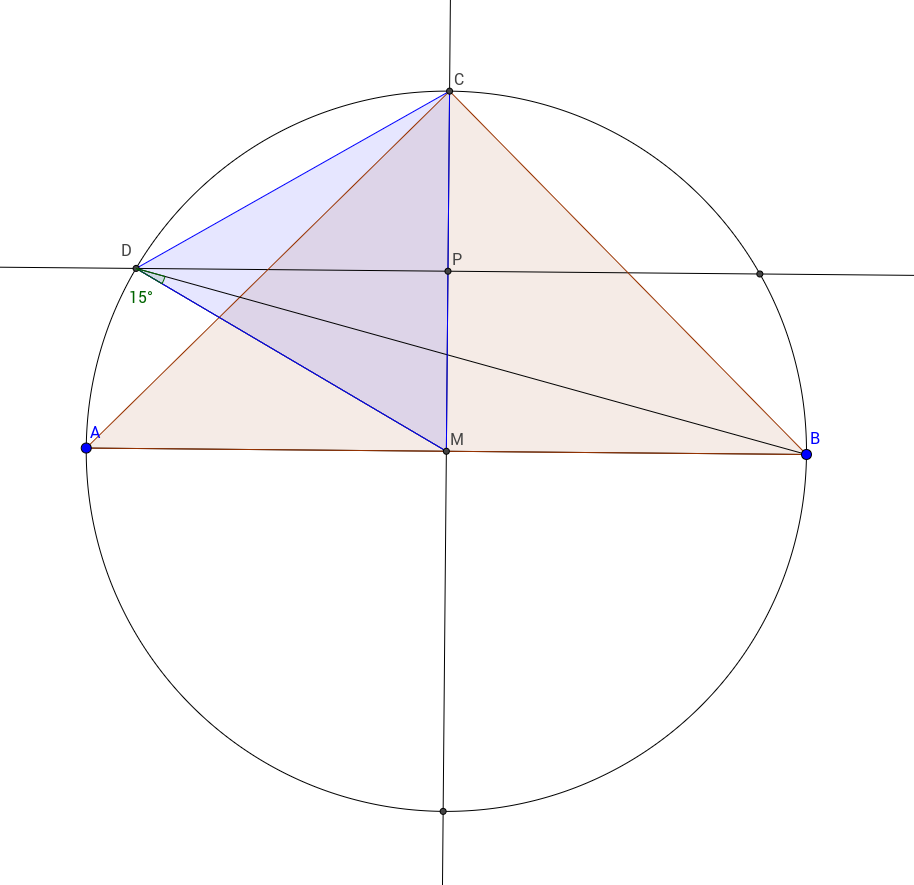
\includegraphics[width=.5\linewidth]{res/KL161-4.png}
\end{figure}

\subsection{Aufgabe} %5
\begin{figure}[H]
	\centering
	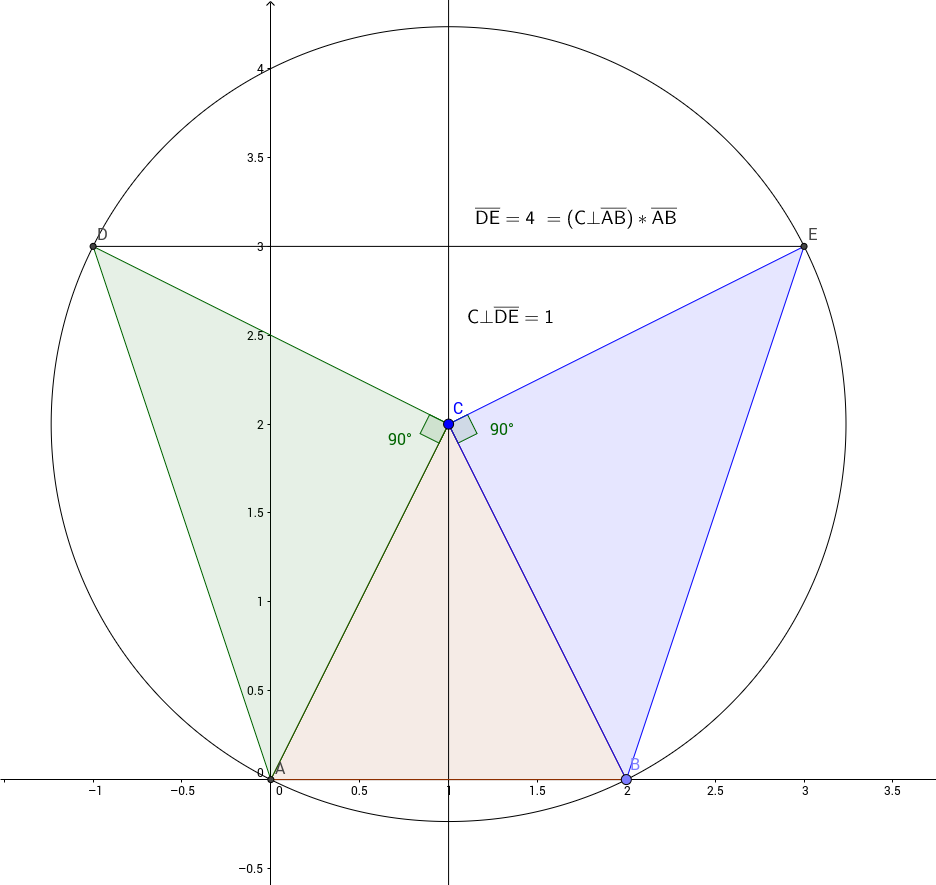
\includegraphics[width=.5\linewidth]{res/KL161-5.png}
\end{figure}

\subsection{Aufgabe} %6
\begin{align*}
\sin(\frac{\alpha}{2}) &= \sqrt{\frac{1 - \cos(\alpha)}{2}} \\
\sin(22.5^\circ) &= \sqrt{\frac{1 - \cos(45^\circ)}{2}} = \sqrt{\frac{1 - \frac{\sqrt{2}}{2}}{2}} = \frac{\sqrt{2 - \sqrt{2}}}{2} \\
\cos(\frac{\alpha}{2}) &= \sqrt{\frac{1 + \cos(\alpha)}{2}} \\
\cos(22.5^\circ) &= \sqrt{\frac{1 + \cos(45^\circ)}{2}} = \sqrt{\frac{1 + \frac{\sqrt{2}}{2}}{2}} = \frac{\sqrt{2 + \sqrt{2}}}{2} \\
\tan(22.5^\circ) &= \frac{\sin(22.5^\circ)}{\cos(22.5^\circ)} = \frac{\frac{\sqrt{2 - \sqrt{2}}}{2}}{\frac{\sqrt{2 + \sqrt{2}}}{2}} = \sqrt{2} - 1
\end{align*}


\end{document}